\documentclass[border=3pt]{standalone}
% Preâmbulo compartilhado pelos diagramas TikZ da aula 14 (SLAM com EIF)
\usepackage[T1]{fontenc}
\usepackage[utf8]{inputenc}
\usepackage{lmodern}
\usepackage{amsmath}
\usepackage{xcolor}
\usepackage{tikz}
\usetikzlibrary{arrows.meta,angles,quotes,decorations.pathmorphing,decorations.pathreplacing,calc,
                positioning,shapes.geometric,shapes.misc,backgrounds,fit,
                math}

% Paleta (mesma dos SVGs originais)
\definecolor{dblue}{HTML}{2A5B8C}
\definecolor{dorange}{HTML}{B3541E}
\definecolor{dgreen}{HTML}{4A7C59}
\definecolor{dred}{HTML}{9C4B4B}
\definecolor{dcream}{HTML}{F4F1EA}
\definecolor{dshade}{HTML}{DDD7C9}

% Função gaussiana (não normalizada por padrão de escala visual)
\pgfmathdeclarefunction{gauss}{3}{%
  \pgfmathparse{1/(#3*sqrt(2*pi))*exp(-((#1-#2)^2)/(2*#3^2))}%
}

% Estilos comuns (prefixo d... para não colidir com chaves internas do pgf)
\tikzset{
  >={Stealth[length=2mm]},
  dguide/.style={gray!55, dashed, line width=0.4pt},
  daxis/.style={gray!60, line width=0.7pt, ->},
  dbody/.style={fill=black!3, draw=black!80, line width=1pt},
  dacc/.style={draw=dblue, line width=1pt},
  dlbl/.style={black!55, font=\small},
  dsub/.style={black!45, font=\footnotesize},
  dstate/.style={circle, draw=black!80, fill=dcream, line width=1pt,
                 minimum size=17mm, font=\large, inner sep=1pt},
  dobs/.style={circle, draw=black!80, fill=dshade, line width=1pt,
               minimum size=14mm, font=\large, inner sep=1pt},
  dbox/.style={rounded corners=2pt, draw=black!80, fill=dcream, line width=1pt,
               align=center, inner sep=6pt},
  dop/.style={circle, draw=black!80, fill=white, line width=1pt,
              minimum size=6mm, inner sep=0pt, font=\small},
  dtrans/.style={->, dblue, line width=1pt},
  dmeas/.style={->, dorange, line width=1pt},
  dcurve/.style={line width=1pt, dblue},
  dcurveb/.style={line width=1.4pt, dorange},
}

\begin{document}
\hyphenpenalty=10000 \exhyphenpenalty=10000 \tolerance=9999 \emergencystretch=3em
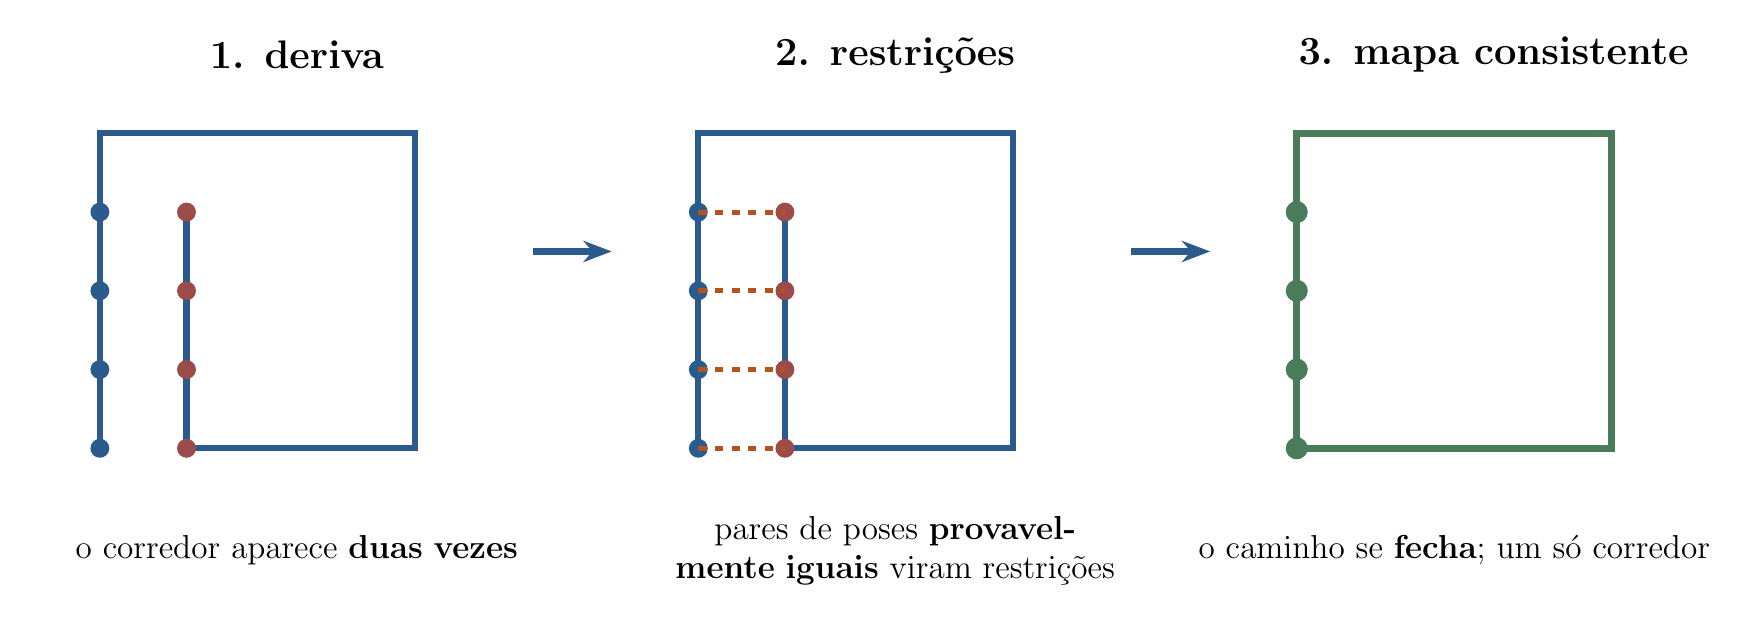
\begin{tikzpicture}[x=1cm,y=1cm]
\tikzset{d/.style={circle, fill=dblue, inner sep=1.4pt}}
\node[font=\Large\bfseries] at (3.0,5.5) {1. deriva};
\draw[dblue, line width=2.2pt] (0.5,0.5) -- (0.5,4.5) -- (4.5,4.5) -- (4.5,0.5) -- (1.6,0.5) -- (1.6,3.6);
\foreach \y in {0.5,1.5,2.5,3.5} {\fill[dblue] (0.5,\y) circle (0.12); \fill[dred] (1.6,\y) circle (0.12);}
\node[font=\large, text width=6.6cm, align=center] at (3.0,-0.8) {o corredor aparece \textbf{duas vezes}};
\node[font=\Large\bfseries] at (10.6,5.5) {2. restrições};
\draw[dblue, line width=2.2pt] (8.1,0.5) -- (8.1,4.5) -- (12.1,4.5) -- (12.1,0.5) -- (9.2,0.5) -- (9.2,3.6);
\foreach \y in {0.5,1.5,2.5,3.5} {\fill[dblue] (8.1,\y) circle (0.12); \fill[dred] (9.2,\y) circle (0.12); \draw[dorange, dashed, line width=1.8pt] (8.1,\y) -- (9.2,\y);}
\node[font=\large, text width=6.6cm, align=center] at (10.6,-0.8) {pares de poses \textbf{provavelmente iguais} viram restrições};
\node[font=\Large\bfseries] at (18.2,5.5) {3. mapa consistente};
\draw[dgreen, line width=2.6pt] (15.7,0.5) -- (15.7,4.5) -- (19.7,4.5) -- (19.7,0.5) -- (15.7,0.5);
\foreach \y in {0.5,1.5,2.5,3.5} {\fill[dgreen] (15.7,\y) circle (0.14);}
\node[font=\large, text width=6.6cm, align=center] at (17.7,-0.8) {o caminho se \textbf{fecha}; um só corredor};
\draw[dtrans, line width=2.4pt, -{Stealth[length=3.6mm]}] (6.0,3.0) -- (7.0,3.0);
\draw[dtrans, line width=2.4pt, -{Stealth[length=3.6mm]}] (13.6,3.0) -- (14.6,3.0);
\end{tikzpicture}
\end{document}
